\documentclass[11pt,a4paper]{report}
\usepackage[T1]{fontenc}
\usepackage{lmodern}
\usepackage[margin=24mm,headheight=15pt]{geometry}
\usepackage{amsmath,amssymb,mathtools,bm,booktabs,longtable,array}
\usepackage{graphicx,xcolor,hyperref,fancyhdr,tikz}
\usetikzlibrary{arrows.meta,positioning,calc}
\definecolor{ink}{HTML}{17324D}
\definecolor{accent}{HTML}{007F87}
\definecolor{soft}{HTML}{E8F2F4}
\hypersetup{colorlinks=true,linkcolor=ink,urlcolor=accent,pdftitle={IntelQcopter: from forces to control and measurements}}
\pagestyle{fancy}\fancyhf{}
\fancyhead[L]{\small\textcolor{ink}{IntelQcopter | Mathematical field guide}}
\fancyhead[R]{\small Derivations and measurements}
\fancyfoot[C]{\thepage}
\setlength{\parindent}{0pt}
\setlength{\parskip}{5pt}
\setlength{\emergencystretch}{3em}
\allowdisplaybreaks
\newcommand{\vect}[1]{\bm{#1}}
\newcommand{\dd}{\,\mathrm d}
\newcommand{\unit}[1]{\,\mathrm{#1}}
\newcommand{\R}{\mathbb R}
\newcommand{\E}{\mathbb E}
\newcommand{\Var}{\operatorname{Var}}
\newcommand{\Cov}{\operatorname{Cov}}
\newcommand{\diag}{\operatorname{diag}}
\newcommand{\crossmat}[1]{[#1]_\times}
\newcommand{\important}[1]{\par\colorbox{soft}{\parbox{\dimexpr\linewidth-2\fboxsep}{#1}}\par}
\title{\Huge\textcolor{ink}{IntelQcopter}\\[8mm]
\LARGE From forces to flight control\\[5mm]
\large A step-by-step nonlinear model, uncertainty and measurement guide}
\author{IntelQcopter project}
\date{20 October 2026}
\begin{document}
\hypersetup{pageanchor=false}
\maketitle
\hypersetup{pageanchor=true}
\pagenumbering{roman}
\chapter*{How to read this guide}
We begin with a force in newtons, explain every symbol, build the full nonlinear
rigid-body equations, then derive local transfer functions for the six existing
controllers. Local models are tools for gain calculation; they do not replace
the nonlinear simulation model.

\important{A calculated value is conditional on its inputs. Our 1.2 kg flight
baseline and separate 0.740 kg component estimate are both unmeasured assumptions.
No number of printed decimal places turns an assumption into a measurement.}

The motor KV label, propeller dimensions and ESC current rating do not identify
thrust gain, delay or inertia. Unknown coefficients remain symbols or explicitly
labelled scenario assumptions until measurements exist.

The current firmware keeps physical motor arming disabled. Its new battery
policy warns at 35 percent estimated charge and latches disarm at 20 percent;
it does not request a controlled landing. If eventually applied in air, motor
thrust is removed and the aircraft falls. Storage and host builds are not
physical flash-endurance or power-loss validation.

\tableofcontents
\clearpage\pagenumbering{arabic}
\chapter{What are we measuring?}
\section{Objects, symbols and units}
A symbol denotes a physical quantity, not an arbitrary number. If a motor
produces $3\unit{N}$, the number 3 depends on the chosen unit; the force itself
does not. Keep units beside measurements and check every equation dimensionally.

\begin{longtable}{@{}p{.17\linewidth}p{.53\linewidth}p{.22\linewidth}@{}}
\toprule Symbol & Meaning & SI unit\\\midrule\endhead
$m$ & Complete aircraft mass, including battery, ESCs and attached parts & kg\\
$\vect r=(x,y,z)^T$ & Position of the aircraft centre of mass in world axes & m\\
$\vect v=\dot{\vect r}$ & Velocity of that centre of mass & m/s\\
$\dot{\vect v}=\ddot{\vect r}$ & Acceleration of that centre of mass & m/s$^2$\\
$g$ & Magnitude of gravitational acceleration; baseline uses 9.80665 & m/s$^2$\\
$T_i$ & Upward body-axis force produced by propeller $i$ & N\\
$T=\sum_iT_i$ & Sum of the four propeller thrust magnitudes & N\\
$R$ & Rotation mapping body components into world components & dimensionless\\
$\vect\omega=(p,q,r_b)^T$ & Body angular velocity; $r_b$ is yaw rate & rad/s\\
$J$ & Inertia tensor about the centre of mass & kg m$^2$\\
$\vect\tau$ & External torque vector about the centre of mass & N m\\
$\Omega_i$ & Rotor spin speed; different from aircraft angular velocity & rad/s\\
$u_i$ & Normalized motor command, before identifying its physical response & dimensionless\\
\bottomrule
\end{longtable}

The dot is a derivative with respect to time:
\begin{align}
\dot x(t)&=\lim_{\epsilon\to0}\frac{x(t+\epsilon)-x(t)}{\epsilon},\\
\ddot x(t)&=\frac{\dd}{\dd t}\dot x(t),\\
\dot{\vect r}&=(\dot x,\dot y,\dot z)^T.
\end{align}
For sampled data separated by $\Delta t$, a finite difference approximates the
derivative. It is an approximation, not the definition:
\begin{equation}
\dot x(t_k)\approx\frac{x_k-x_{k-1}}{\Delta t}.
\end{equation}

\section{Mass is not weight; thrust is a force}
Mass describes inertia against translational acceleration. Weight is the
gravitational force. Their relationship is
\begin{equation}
W=mg,\qquad [W]=\unit{kg}\frac{\unit m}{\unit{s^2}}=\unit N.
\end{equation}
A propeller accelerates air downward; the aerodynamic reaction exerts an upward
force on the motor/airframe. That force magnitude is its thrust $T_i$.
It is not a temperature, a torque, a throttle percentage or a mass.

For four parallel propeller axes, expressed in body coordinates,
\begin{align}
\vect F_{1,B}&=(0,0,T_1)^T,&
\vect F_{2,B}&=(0,0,T_2)^T,\\
\vect F_{3,B}&=(0,0,T_3)^T,&
\vect F_{4,B}&=(0,0,T_4)^T.
\end{align}
Forces add component by component:
\begin{align}
\vect F_{T,B}
&=\vect F_{1,B}+\vect F_{2,B}+\vect F_{3,B}+\vect F_{4,B}\\
&=\begin{bmatrix}0+0+0+0\\0+0+0+0\\T_1+T_2+T_3+T_4\end{bmatrix}\\
&=\begin{bmatrix}0\\0\\T\end{bmatrix},
\qquad \boxed{T=T_1+T_2+T_3+T_4}.
\end{align}
Only the propeller axes being parallel permits this particular scalar sum.
For tilted rotor axes $\vect n_{i,B}$, the general expression is
$\vect F_{T,B}=\sum_i T_i\vect n_{i,B}$.

\begin{figure}[ht]
\centering
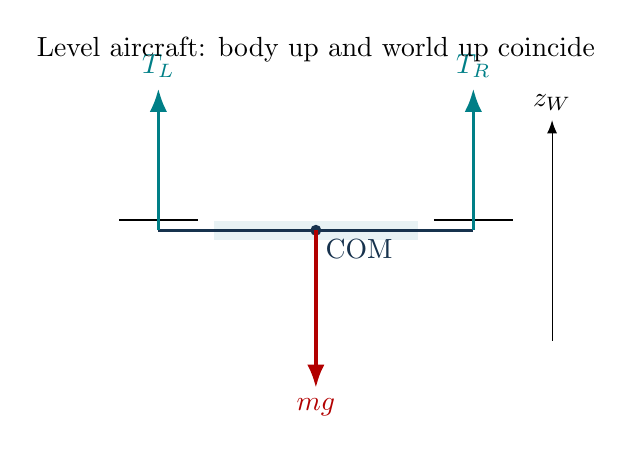
\begin{tikzpicture}[>=Latex,scale=1]
\fill[soft] (-1.3,-.12) rectangle (1.3,.12);
\draw[very thick,ink] (-2,0)--(2,0);
\draw[thick] (-2.5,.13)--(-1.5,.13) (1.5,.13)--(2.5,.13);
\fill[ink] (0,0) circle (.07) node[below right]{COM};
\draw[->,very thick,accent] (-2,0)--(-2,1.8) node[above]{$T_L$};
\draw[->,very thick,accent] (2,0)--(2,1.8) node[above]{$T_R$};
\draw[->,very thick,red!70!black] (0,0)--(0,-2) node[below]{$mg$};
\draw[->] (3,-1.4)--(3,1.4) node[above]{$z_W$};
\node at (0,2.3){Level aircraft: body up and world up coincide};
\end{tikzpicture}
\caption{Side view groups two rotors per side. All arrows are forces; the COM
is the point used for translation and torque accounting.}
\end{figure}

\section{One vector, two coordinate descriptions}
The world frame is fixed for a local experiment. The body frame rotates with
the aircraft. Body x points forward, y left, z up. A vector must be expressed in
one common frame before adding it to another vector.

Let $\vect b_1,\vect b_2,\vect b_3$ be the body unit axes, each expressed in world
coordinates. Define
\begin{equation}
R=\begin{bmatrix}|&|&|\\\vect b_1&\vect b_2&\vect b_3\\|&|&|\end{bmatrix}.
\end{equation}
For body components $(f_x,f_y,f_z)$, the physical vector is
\begin{align}
\vect F_W&=f_x\vect b_1+f_y\vect b_2+f_z\vect b_3\\
&=R\begin{bmatrix}f_x\\f_y\\f_z\end{bmatrix}.
\end{align}
Because the axes are orthonormal,
\begin{equation}
R^TR=I,\qquad R^{-1}=R^T,\qquad \det R=+1.
\end{equation}
Consequently $\vect F_B=R^T\vect F_W$. Multiplying by $R$ changes components,
not force magnitude: $\|R\vect F_B\|=\|\vect F_B\|$.

\section{Build the rotation explicitly}
Use roll $\phi$, pitch $\theta$ and yaw $\psi$, with the convention
$R=R_z(\psi)R_y(\theta)R_x(\phi)$. All trigonometric arguments here are radians.
\begin{align}
R_x(\phi)&=\begin{bmatrix}1&0&0\\0&\cos\phi&-\sin\phi\\0&\sin\phi&\cos\phi\end{bmatrix},\\
R_y(\theta)&=\begin{bmatrix}\cos\theta&0&\sin\theta\\0&1&0\\-\sin\theta&0&\cos\theta\end{bmatrix},\\
R_z(\psi)&=\begin{bmatrix}\cos\psi&-\sin\psi&0\\\sin\psi&\cos\psi&0\\0&0&1\end{bmatrix}.
\end{align}
We only need the rotated thrust direction, so start with
$\vect e_3=(0,0,1)^T$ and perform each physical rotation:
\begin{align}
R_x\vect e_3&=\begin{bmatrix}0\\-\sin\phi\\\cos\phi\end{bmatrix},\\
R_yR_x\vect e_3&=\begin{bmatrix}\sin\theta\cos\phi\\-\sin\phi\\\cos\theta\cos\phi\end{bmatrix},\\
R\vect e_3&=\begin{bmatrix}
\cos\psi\sin\theta\cos\phi+\sin\psi\sin\phi\\
\sin\psi\sin\theta\cos\phi-\cos\psi\sin\phi\\
\cos\theta\cos\phi
\end{bmatrix}.
\end{align}
The last vector is exactly the third column of $R$. Thus the world thrust is
$T$ times this column. We have not used $\sin\phi\approx\phi$ or any small-angle
approximation.

\chapter{Where the translational equation comes from}
\section{Start with Newton's law}
For constant mass, linear momentum is $\vect P=m\vect v$. The momentum balance is
\begin{align}
\frac{\dd\vect P}{\dd t}&=\sum\vect F_{\rm external},\\
\frac{\dd(m\vect v)}{\dd t}&=\sum\vect F_{\rm external},\\
m\dot{\vect v}&=\sum\vect F_{\rm external}.
\end{align}
If mass changes, the second line needs more careful momentum accounting; battery
discharge does not meaningfully eject aircraft mass in our model.

List every force and express it in world axes:
\begin{align}
\vect F_{T,W}&=R(0,0,T)^T&&\text{propellers},\\
\vect F_{g,W}&=(0,0,-mg)^T&&\text{gravity},\\
\vect F_{D,W}&=-d\vect v&&\text{current simple drag assumption},\\
\vect F_{{dist},W}&=\text{other unmodelled external forces}.
\end{align}
Substitute these four expressions into Newton's law:
\begin{align}
m\dot{\vect v}
&=\vect F_{T,W}+\vect F_{g,W}+\vect F_{D,W}+\vect F_{{dist},W}\\
&=\boxed{R\begin{bmatrix}0\\0\\T\end{bmatrix}
-\begin{bmatrix}0\\0\\mg\end{bmatrix}
-d\vect v+\vect F_{\rm dist}}.
\end{align}
This is the requested equation. It is a force balance, not a guessed controller
formula. Every term has units of newtons:
\begin{equation}
[m\dot v]=\unit N,\quad [RT]=\unit N,\quad [mg]=\unit N,\quad
[d]=\unit{N\,s/m},\quad[dv]=\unit N.
\end{equation}

\section{Write each differential equation without hiding $R$}
Using the third-column expression derived earlier:
\begin{align}
m\ddot x&=T(\cos\psi\sin\theta\cos\phi+\sin\psi\sin\phi)-d\dot x+f_x,\\
m\ddot y&=T(\sin\psi\sin\theta\cos\phi-\cos\psi\sin\phi)-d\dot y+f_y,\\
m\ddot z&=T\cos\theta\cos\phi-mg-d\dot z+f_z.
\end{align}
These are coupled nonlinear equations because of products of changing thrust
and trigonometric functions of changing attitude.

At level hover, $\phi=\theta=0$, $\vect v=0$ and disturbances are neglected:
\begin{align}
0&=T-mg,&T&=mg,&T_i&=\frac{mg}{4}\quad\text{if balanced}.
\end{align}
For the assumed $m=1.2\unit{kg}$:
\begin{equation}
mg=11.76798\unit N,\qquad T_i=2.941995\unit N.
\end{equation}
At roll $30^\circ$, pitch zero and zero vertical acceleration:
\begin{align}
T\cos30^\circ&=mg,&
T&=\frac{mg}{\cos30^\circ}\approx13.5885\unit N.
\end{align}
The larger total thrust is needed because some thrust now points horizontally.
Keeping $T=mg$ while tilting instead gives downward vertical acceleration.

\section{A more general aerodynamic force model}
The force balance remains exact as an accounting statement; a chosen drag law
can still be approximate. A richer candidate is
\begin{align}
\vect v_{\rm rel}&=\vect v_W-\vect w_W,\\
\vect F_D&=-D_1\vect v_{\rm rel}
-D_2\bigl(\|\vect v_{\rm rel}\|\vect v_{\rm rel}\bigr).
\end{align}
$\vect w_W$ is wind velocity. $D_1,D_2$ may depend on attitude and direction.
Their coefficients need data. Adding unknown coefficients without measurement
does not automatically make a simulation more accurate.

\section{After commanded disarming}
Disarming removes commanded rotor drive; the rotor does not physically stop
spinning at the exact same instant. Its motor/air dynamics determine spin-down.
As $T\to0$, neglecting drag for this illustration,
\begin{align}
\ddot z&=-g,\\
\dot z(t)&=v_{z0}-gt,\\
z(t)&=z_0+v_{z0}t-\tfrac12gt^2.
\end{align}
These equations describe falling, not a controlled landing. The selected
20-percent battery action requests this motor inhibition regardless of height.

\chapter{Why rotation needs an inertia tensor}
\section{Torque comes from force and lever arm}
For a force $\vect F$ applied at displacement $\vect r_i$ from the centre of mass,
\begin{equation}
\vect\tau_i=\vect r_i\times\vect F_i.
\end{equation}
For $\vect a=(a_x,a_y,a_z)^T$ and $\vect b=(b_x,b_y,b_z)^T$,
\begin{equation}
\vect a\times\vect b=
\begin{bmatrix}a_yb_z-a_zb_y\\a_zb_x-a_xb_z\\a_xb_y-a_yb_x\end{bmatrix}.
\end{equation}
This operation is the vector cross product. Its magnitude is
$\|\vect a\|\|\vect b\|\sin\gamma$ and its direction follows the right-hand rule.
It is not component-by-component multiplication.

For a rotor at $(x_i,y_i,z_i)$ with upward thrust $(0,0,T_i)$,
\begin{equation}
\vect\tau_{T,i}=
\begin{bmatrix}y_iT_i\\-x_iT_i\\0\end{bmatrix}.
\end{equation}
A rotor far from the centre creates a greater roll/pitch torque for the same
thrust. Its vertical height $z_i$ does not appear for this parallel upward force.

\section{Build angular momentum from individual mass elements}
For a mass element $\dd m$ at body position $\vect\rho$, rigid-body rotation
produces velocity $\vect\omega\times\vect\rho$ relative to the centre. Its angular
momentum about the centre is
\begin{align}
\dd\vect H&=\vect\rho\times(\vect\omega\times\vect\rho)\dd m\\
&=\bigl[(\vect\rho^T\vect\rho)I-\vect\rho\vect\rho^T\bigr]\vect\omega\dd m.
\end{align}
Integrate over the entire assembled body:
\begin{align}
\vect H_B&=J\vect\omega,\\
J&=\int\left(\|\vect\rho\|^2I-\vect\rho\vect\rho^T\right)\dd m\\
&=\begin{bmatrix}
\int(y^2+z^2)\dd m&-\int xy\dd m&-\int xz\dd m\\
-\int xy\dd m&\int(x^2+z^2)\dd m&-\int yz\dd m\\
-\int xz\dd m&-\int yz\dd m&\int(x^2+y^2)\dd m
\end{bmatrix}.
\end{align}
$J_x$ therefore measures resistance to angular acceleration around body x.
It depends on where mass is located, not only the total mass. Moving a battery
away from an axis increases inertia about that axis.

\section{Derive the rotating-frame derivative}
Let a physical vector have body components $\vect H_B$ and world components
$\vect H_W=R\vect H_B$. Differentiate with the product rule:
\begin{align}
\dot{\vect H}_W&=\dot R\vect H_B+R\dot{\vect H}_B.
\end{align}
Rotation kinematics gives $\dot R=R\crossmat{\vect\omega}$, where
\begin{equation}
\crossmat{\vect\omega}=
\begin{bmatrix}0&-r_b&q\\r_b&0&-p\\-q&p&0\end{bmatrix},
\qquad \crossmat{\vect\omega}\vect H_B=\vect\omega\times\vect H_B.
\end{equation}
Thus
\begin{align}
\dot{\vect H}_W
&=R\left(\dot{\vect H}_B+\vect\omega\times\vect H_B\right).
\end{align}
Angular-momentum balance says $\dot{\vect H}_W=\vect\tau_W$.
Multiply by $R^T$:
\begin{align}
\vect\tau_B&=\dot{\vect H}_B+\vect\omega\times\vect H_B.
\end{align}
For constant inertia, $\dot{\vect H}_B=J\dot{\vect\omega}$. Substitute
$\vect H_B=J\vect\omega$:
\begin{align}
\vect\tau_B&=J\dot{\vect\omega}+\vect\omega\times(J\vect\omega),\\
J\dot{\vect\omega}
&=\vect\tau_B-\vect\omega\times(J\vect\omega).
\end{align}
The cross term accounts for the body axes themselves rotating while the angular
momentum vector is described in those axes. It is not an extra arbitrary torque.

\section{Expand the nonlinear coupling}
If the selected body axes are principal axes,
$J=\diag(J_x,J_y,J_z)$ and
\begin{align}
J\vect\omega&=(J_xp,J_yq,J_zr_b)^T,\\
\vect\omega\times(J\vect\omega)
&=\begin{bmatrix}
(J_z-J_y)qr_b\\(J_x-J_z)pr_b\\(J_y-J_x)pq
\end{bmatrix}.
\end{align}
Subtract each component and divide by its inertia:
\begin{align}
\dot p&=\frac{\tau_x+(J_y-J_z)qr_b}{J_x},\\
\dot q&=\frac{\tau_y+(J_z-J_x)r_bp}{J_y},\\
\dot r_b&=\frac{\tau_z+(J_x-J_y)pq}{J_z}.
\end{align}
For a non-diagonal measured tensor, use the full matrix inverse or solve
$J\dot{\vect\omega}=\cdots$; do not delete products of inertia just for convenience.

\section{Angle derivatives are not generally gyro components}
For the stated Euler convention,
\begin{equation}
\begin{bmatrix}\dot\phi\\\dot\theta\\\dot\psi\end{bmatrix}=
\begin{bmatrix}
1&\sin\phi\tan\theta&\cos\phi\tan\theta\\
0&\cos\phi&-\sin\phi\\
0&\sin\phi/\cos\theta&\cos\phi/\cos\theta
\end{bmatrix}
\begin{bmatrix}p\\q\\r_b\end{bmatrix}.
\end{equation}
Only near modest attitudes/rates can $\dot\phi\approx p$ and $\dot\theta\approx q$
be substituted conveniently. The current independent angle/bias filters use that
approximation; the physical rotational model need not.

To avoid the Euler singularity at $\cos\theta=0$, propagate a unit quaternion.
For body-to-world quaternion $q=(q_w,q_x,q_y,q_z)$,
\begin{equation}
\dot q=\frac12 q\otimes(0,p,q_{\rm rate},r_b),\qquad \|q\|=1.
\end{equation}
Here $q_{\rm rate}$ means the gyro y rate, not the quaternion. A numerical
implementation must keep these two meanings distinct and normalize as needed.

\chapter{The four rotors and the nonlinear actuator model}
\section{Geometry and force allocation}
For motor diagonal $D$ in an X layout, $a=D/(2\sqrt2)$:
\begin{equation}
(x_i,y_i)=
(a,a),(a,-a),(-a,-a),(-a,a)
\end{equation}
in order FL, FR, RR, RL.
\begin{figure}[ht]
\centering
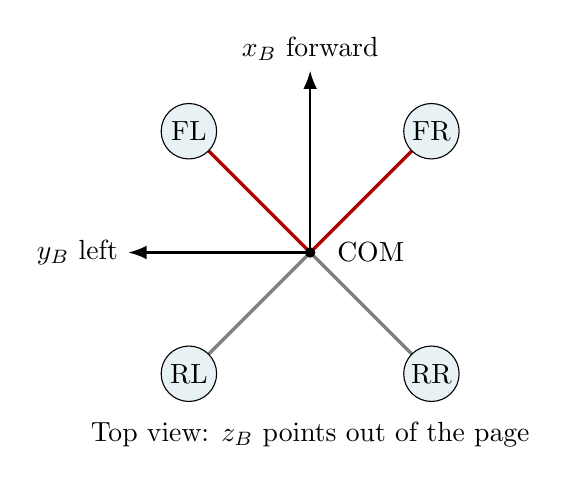
\begin{tikzpicture}[>=Latex,scale=1.1]
\draw[very thick,red!70!black] (0,0)--(-1.4,1.4) (0,0)--(1.4,1.4);
\draw[very thick,gray] (0,0)--(-1.4,-1.4) (0,0)--(1.4,-1.4);
\foreach \x/\y/\name in {-1.4/1.4/FL,1.4/1.4/FR,1.4/-1.4/RR,-1.4/-1.4/RL}{
\draw[fill=soft] (\x,\y) circle (.32); \node at (\x,\y){\name};}
\draw[->,thick] (0,0)--(0,2.1) node[above]{$x_B$ forward};
\draw[->,thick] (0,0)--(-2.1,0) node[left]{$y_B$ left};
\fill (0,0) circle (.06);
\node[right] at (.2,0){COM};
\node at (0,-2.1){Top view: $z_B$ points out of the page};
\end{tikzpicture}
\caption{Logical geometry; verify actual wiring, arm orientation and propeller
spin before assigning a physical motor number.}
\end{figure}
With reaction torque $Q_i=\kappa T_i$ and the selected yaw signs:
\begin{equation}
\begin{bmatrix}T\\\tau_x\\\tau_y\\\tau_z\end{bmatrix}=
\begin{bmatrix}
1&1&1&1\\a&-a&-a&a\\-a&-a&a&a\\-\kappa&\kappa&-\kappa&\kappa
\end{bmatrix}
\begin{bmatrix}T_{FL}\\T_{FR}\\T_{RR}\\T_{RL}\end{bmatrix}.
\end{equation}
This allocation is a geometric consequence of $\vect r\times\vect F$ plus yaw
reaction signs. A physically measured $Q_i(\Omega_i)$ can replace the constant
$\kappa$ model.

\section{Retain speed-squared thrust}
A common aerodynamic form is
\begin{equation}
T_i=k_T\Omega_i^2,\qquad Q_i=k_Q\Omega_i^2.
\end{equation}
More generally $k_T,k_Q$ depend on inflow, propeller condition, density and advance
ratio. These functions are not identified from a 9047 label alone.

An effective motor/ESC model can be written
\begin{align}
L\dot I_i&=V_{{eff},i}-R_m I_i-k_e\Omega_i,\\
J_r\dot\Omega_i&=k_\tau I_i-Q_i(\Omega_i)-B_r\Omega_i,\\
V_{{eff},i}&=\mu(u_i,V_{\rm pack},\hbox{ESC settings})V_{\rm pack}.
\end{align}
The ESC is an electronic commutator, so these are effective averaged equations;
phase/line voltage conventions and efficiency must be specified before interpreting
$k_e,k_\tau$. Do not silently equate a PWM input percentage with an effective
phase voltage or a thrust percentage.

The KV rating indicates an approximate no-load speed/voltage relationship.
It does not supply $R_m,L,J_r,k_T,k_Q$, loaded RPM, ESC map $\mu$, or transient
delay. We therefore retain these coefficients symbolically until measurement.

\section{Rotor angular momentum: optional additional physics}
If $\sigma_i=\pm1$ denotes rotor spin direction,
\begin{equation}
\vect H_{\rm rot}=\sum_i\sigma_iJ_r\Omega_i\vect e_3.
\end{equation}
For an assembled-airframe inertia $J$ defined for frozen relative rotor angles,
the total rotating-body momentum balance can be expanded as
\begin{equation}
J\dot{\vect\omega}
=\vect\tau_{\rm external}
-\vect\omega\times(J\vect\omega)
-\dot{\vect H}_{\rm rot}
-\vect\omega\times\vect H_{\rm rot}.
\end{equation}
External rotor aerodynamic drag has sign opposite $\sigma_i$; if using the
usual body reaction-torque sign $s_i$, then $s_i=-\sigma_i$.
Do not count the same motor/rotor torque twice by adding it both as an external
reaction and as an internal rotor acceleration contribution.

These extra terms need rotor inertia/spin information. They are model extensions,
not claims that the present Gazebo adapter has identified or enabled them.

\section{Battery and actuator coupling}
A symbolic electrical extension is
\begin{align}
V_{\rm term}&=V_{\rm oc}(z,T_b)-I_{\rm pack}R_0-V_p,\\
\dot V_p&=-\frac{V_p}{R_1C_1}+\frac{I_{\rm pack}}{C_1},\\
\dot z&=-\frac{\eta(I_{\rm pack},T_b)I_{\rm pack}}{3600C_{\rm eff}},
\qquad z\in[0,1].
\end{align}
$C_{\rm eff}$ is in Ah and positive current means discharge. Phase motor currents
are not automatically identical to pack current; inverter efficiency and duty
matter. Voltage sag changes available speed/thrust, connecting electrical and
mechanical dynamics.

\important{For current reproducible flight results, the adapter still uses
declared first-order thrust lag and normalized linear thrust, while Gazebo
integrates nonlinear rigid-body/contact dynamics. The richer equations above
define the model to identify; no arbitrary electrical coefficients were invented
or silently substituted into an already-recorded flight.}

\section{Why a single transfer function cannot represent all of this}
Transfer functions describe linear time-invariant input/output models with
specified initial conditions. Our exact equations contain $\Omega^2$,
$T\cos\phi\cos\theta$, and $pq$ products. In general,
\begin{equation}
\mathcal L\{\Omega(t)^2\}\ne\bigl(\mathcal L\{\Omega(t)\}\bigr)^2.
\end{equation}
We use the nonlinear equations for prediction and simulation, and a local
Jacobian model for transfer-function/gain design. Multiple operating points or
nonlinear control methods can extend this design later; pretending the full
nonlinear aircraft has one global scalar transfer function would be incorrect.

\chapter{Equilibrium, local models and the six controllers}
\section{Keep the full model as the prediction model}
Collect the nonlinear mechanical, rotor and electrical states:
\begin{equation}
\vect x=(\vect r^T,\vect v^T,q^T,\vect\omega^T,
\Omega_1,\ldots,\Omega_4,I_1,\ldots,I_4,V_p,z)^T.
\end{equation}
The preceding equations define $\dot{\vect x}=f(\vect x,\vect u,\vect\theta)$,
where $\vect\theta$ contains measured or assumed physical parameters. The unit
quaternion has one constraint. A numerical simulation integrates these equations;
it need not replace trigonometric functions with their small-angle forms.

For controller calculation, select a level hover operating point:
\begin{align}
\vect v_0&=0,&\vect\omega_0&=0,&R_0&=I,\\
\sum_i k_T\Omega_{i0}^2&=mg,&
k_\tau I_{i0}&=Q_i(\Omega_{i0})+B_r\Omega_{i0}.
\end{align}
For symmetric rotors, $\Omega_{i0}=\sqrt{mg/(4k_T)}$.
Without identified $k_T$, this is a relationship, not an available numeric RPM.

\section{Where a local linear model comes from}
Write $\vect x=\vect x_0+\delta\vect x$ and $\vect u=\vect u_0+\delta\vect u$.
A first-order Taylor expansion at equilibrium gives
\begin{align}
f(\vect x_0+\delta\vect x,\vect u_0+\delta\vect u)
&=f(\vect x_0,\vect u_0)
+A\delta\vect x+B\delta\vect u+\text{higher-order terms},\\
A&=\left.\frac{\partial f}{\partial\vect x}\right|_0,&
B&=\left.\frac{\partial f}{\partial\vect u}\right|_0.
\end{align}
At equilibrium $f(\vect x_0,\vect u_0)=0$. Neglecting only the remainder gives
the \emph{local} perturbation model. This step is explicitly labelled and does
not delete the original nonlinear equations.

For example, speed-squared thrust expands exactly as
\begin{align}
T(\Omega_0+\delta\Omega)
&=k_T\Omega_0^2+2k_T\Omega_0\delta\Omega+k_T(\delta\Omega)^2,\\
\delta T&\approx 2k_T\Omega_0\delta\Omega.
\end{align}
The local slope $2k_T\Omega_0$ changes with operating point.
For a measured command curve $T=f_T(u)$,
$\delta T\approx f_T'(u_0)\delta u$. A nonlinear thrust curve can therefore be
used for simulation while its measured hover slope supplies local controller gain.

\section{The currently reproducible baseline}
\begin{center}
\begin{tabular}{@{}ll@{}}\toprule
Parameter & Assumed baseline\\\midrule
$m$ & 1.2 kg\\
$(J_x,J_y,J_z)$ & (.012,.012,.022) kg m$^2$\\
$D$, $a=D/(2\sqrt2)$ & .45 m, .159099 m\\
$T_{\max}$ & 6 N per rotor in the normalized linear-thrust surrogate\\
$\tau_m$ & .04 s thrust lag\\
$d$ & .12 N s/m\\
$\Delta t$ & .002 s virtual control interval\\\bottomrule
\end{tabular}
\end{center}
For the surrogate $T_i=T_{\max}u_i^a$,
\begin{equation}
c_0=\frac{mg}{4T_{\max}}=.4903325.
\end{equation}
The other model is the provisional .740 kg component URDF, with inertia
\begin{equation}
(J_x,J_y,J_z)=(.00885852,.00906322,.01718682)\unit{kg\,m^2}.
\end{equation}
Its masses are not verified and it is
not the physics body of the recorded 1.2 kg flight. Never combine one model's
mass with another model's inertia accidentally.

\section{Derive each local transfer function}
For a small roll perturbation, with other rates zero,
\begin{align}
J_x\dot p&=4aT_{\max}u_\phi^a,\\
\tau_m\dot u_\phi^a+u_\phi^a&=u_\phi.
\end{align}
In radian units define $b_x=4aT_{\max}/J_x$. Under zero perturbation initial
conditions, $\mathcal L\{\dot p\}=sP(s)$, so
\begin{align}
sP(s)&=b_xU_\phi^a(s),\\
(\tau_ms+1)U_\phi^a(s)&=U_\phi(s),\\
\frac{P(s)}{U_\phi(s)}&=\frac{b_x}{s(\tau_ms+1)}.
\end{align}
Integrating rate gives a further factor $1/s$ in the local angle plant:
\begin{equation}
G_\phi(s)=\frac{b_x}{s^2(\tau_ms+1)}.
\end{equation}
Pitch substitutes $J_y$. Yaw rate substitutes $b_z=4\kappa T_{\max}/J_z$ and
has no outer yaw-angle controller.

The present C rate inputs are degrees/s. Multiply the radian effectiveness by
$180/\pi$ before using those C gain units:
\begin{equation}
b_{\phi,\deg}=18231.4054,\qquad b_{\psi,\deg}=937.5673.
\end{equation}
For height, subtract hover equilibrium and set $\lambda=d/m$:
\begin{align}
\delta\ddot h+\lambda\delta\dot h&=b_h\delta c^a,&b_h&=\frac{4T_{\max}}m,\\
G_h(s)&=\frac{b_h}{s(s+\lambda)(\tau_ms+1)}.
\end{align}
The numeric baseline is
$G_h(s)=20/[s(s+.1)(.04s+1)]$.

\section{Why do not all controllers use nonzero P, I and D?}
The letters name three available mathematical terms:
\begin{align}
e(t)&=r(t)-y(t),\\
u_P(t)&=K_pe(t),\\
u_I(t)&=K_i\int_0^t e(\xi)\dd\xi,\\
u_D(t)&=-K_d\dot y(t).
\end{align}
The last form differentiates measurement to avoid target-derivative kick.
Choosing $K_i=0$ or $K_d=0$ is a design choice, not an incomplete calculation.

\subsection{P changes the immediate response}
Larger error gives larger correction. For an angle error of 3 degrees and outer
$K_a=3\unit{s^{-1}}$, the desired rate is 9 degrees/s. P-only angle control can
work with an inner rate PI that rejects constant torque disturbances.

\subsection{I adds a state and removes certain steady errors}
For a constant rate disturbance, the inner rate integral can grow until its
output balances the disturbance torque. But each integrator adds dynamic order
and can accumulate unavailable demand during saturation. An additional outer
angle integral is not automatically beneficial; sensor bias is not made physically
correct merely by integrating its mistaken measurement.

\subsection{D amplifies high-frequency measurement variation}
If independent measurement noise has variance $\sigma_y^2$,
\begin{align}
\dot y_k&\approx(y_k-y_{k-1})/\Delta t,\\
\Var(\dot n_k)&=\frac{2\sigma_y^2}{\Delta t^2}.
\end{align}
At .2 degrees/s gyro sigma and .002 s spacing, the unfiltered rate derivative
noise sigma would be about $141.4$ degrees/s$^2$. Real filtering/correlation
changes that number, but not the need to account for noise. A nonzero rate D
term therefore needs bandwidth/noise design, not merely a wish to use all letters.

\subsection{Why altitude does use D}
The altitude controller has a useful filtered velocity estimate. It forms
\begin{equation}
u_h=K_p(h_{\rm ref}-\hat h)+K_iI_h+K_d(v_{\rm cmd}-\hat v).
\end{equation}
Since $\dot h_{\rm ref}\approx v_{\rm cmd}$ away from its limiter, the last term
is a derivative of height error using an estimated state rather than a noisy
finite difference. There is one altitude PID, not a seventh separate velocity PID.

\section{Calculate the initial six gains}
For a rate plant first approximated by $b/s$, use PI:
\begin{align}
C(s)&=\frac{K_ps+K_i}{s},\\
1+C(s)G(s)&=0,\\
s^2+bK_ps+bK_i&=0.
\end{align}
Choose $s^2+2\zeta\omega_ns+\omega_n^2$ and equate coefficients:
\begin{equation}
K_p=\frac{2\zeta\omega_n}{b},\qquad
K_i=\frac{\omega_n^2}{b}.
\end{equation}
For the current candidate, $\zeta=.9$, roll/pitch $\omega_n=8.4$ rad/s,
yaw $\omega_n=2.8$ rad/s, and outer angle $K_a=3$.
These bandwidths are chosen response objectives, not motor measurements.

For the initial altitude double-integrator design,
\begin{align}
G(s)&=b_h/s^2,\\
1+\left(K_p+K_i/s+K_ds\right)G(s)&=0,\\
s^3+b_hK_ds^2+b_hK_ps+b_hK_i&=0.
\end{align}
Expand desired $(s+p_h)(s^2+2\zeta_h\omega_hs+\omega_h^2)$:
\begin{align}
s^3+(2\zeta_h\omega_h+p_h)s^2
+(\omega_h^2+2\zeta_h\omega_hp_h)s+p_h\omega_h^2.
\end{align}
Coefficient matching gives
\begin{equation}
K_d=\frac{2\zeta_h\omega_h+p_h}{b_h},\quad
K_p=\frac{\omega_h^2+2\zeta_h\omega_hp_h}{b_h},\quad
K_i=\frac{p_h\omega_h^2}{b_h}.
\end{equation}
Use $\omega_h=1.05$, $p_h=.56$, $\zeta_h=.9$. The resulting degree-based C gains:
\begin{center}
\begin{tabular}{@{}lrrr@{}}\toprule
Loop & $K_p$ & $K_i$ & $K_d$\\\midrule
Roll angle & 3 & 0 & 0\\
Roll rate & .0008293381 & .0038702447 & 0\\
Pitch angle & 3 & 0 & 0\\
Pitch rate & .0008293381 & .0038702447 & 0\\
Yaw rate & .0053756141 & .0083620664 & 0\\
Altitude & .108045 & .03087 & .1225\\\bottomrule
\end{tabular}
\end{center}

\section{Now restore lag, drag and the complete cascade}
For a rate PI with lag, the characteristic is
\begin{equation}
\tau_ms^3+s^2+bK_ps+bK_i.
\end{equation}
Positive gains are not enough: the cubic Routh condition also requires
$K_p>\tau_mK_i$. The baseline roll/pitch polynomial is
$.04s^3+s^2+15.12s+70.56$, with poles $-7$ and $-9\pm13.0767j$.

The outer angle loop surrounds the closed inner rate loop plus angle integration:
\begin{align}
T_p(s)&=\frac{b(K_ps+K_i)}{\tau_ms^3+s^2+bK_ps+bK_i},\\
1+\frac{K_aT_p(s)}s&=0.
\end{align}
Multiplying out gives the complete cascade characteristic
\begin{equation}
\tau_ms^4+s^3+bK_ps^2+b(K_i+K_aK_p)s+K_abK_i.
\end{equation}
For altitude with drag and lag:
\begin{equation}
\tau_ms^4+(1+\tau_m\lambda)s^3+(\lambda+b_hK_d)s^2+b_hK_ps+b_hK_i.
\end{equation}
These quartics retain more of the local dynamics than the initial simplified
coefficient-matching models.

For $a_4s^4+a_3s^3+a_2s^2+a_1s+a_0$, the Routh first-column construction is
\begin{align}
b_1&=\frac{a_3a_2-a_4a_1}{a_3},\\
c_1&=\frac{b_1a_1-a_3a_0}{b_1}.
\end{align}
With all $a_i>0$, positivity reduces to
\begin{align}
\Delta_2&=a_3a_2-a_4a_1>0,\\
\Delta_3&=a_3a_2a_1-a_4a_1^2-a_3^2a_0>0.
\end{align}
For the baseline angle cascade these are 10.4832 and 1003.532544.
For altitude they are 2.473764 and 4.7232075492. Both local continuous models
satisfy the conditions; this does not prove a delayed/saturated nonlinear flight.

\subsection{A fuller altitude coefficient match}
Choose the fourth-order desired polynomial
\begin{equation}
\tau_m(s+\rho)(s+p_h)(s^2+2\zeta_h\omega_hs+\omega_h^2).
\end{equation}
The cubic coefficient fixes
$\rho=1/\tau_m+\lambda-p_h-2\zeta_h\omega_h$. Equate the other coefficients:
\begin{align}
K_d&=\frac{\tau_m[\omega_h^2+2\zeta_h\omega_hp_h+
\rho(p_h+2\zeta_h\omega_h)]-\lambda}{b_h},\\
K_p&=\frac{\tau_m[p_h\omega_h^2+
\rho(\omega_h^2+2\zeta_h\omega_hp_h)]}{b_h},\\
K_i&=\frac{\tau_m\rho p_h\omega_h^2}{b_h}.
\end{align}
This gives the uninstalled analytic candidate
$(.09912357,.02796822,.1103068)$ for $(K_p,K_i,K_d)$.
It has selected local poles $-22.65$, $-.56$, $-.945\pm.457684j$.
It has not replaced the recorded-flight gains or been verified in a new flight.

\section{Sampling, limits and nonlinear assessment}
For a local continuous state model, zero-order-hold discretization is
\begin{equation}
A_d=e^{A\Delta t},\qquad B_d=\int_0^{\Delta t}e^{A\xi}B\dd\xi.
\end{equation}
Augment the discrete plant with integral, estimator and delay states. Local
sampled stability requires all closed-loop eigenvalues to satisfy $|z_i|<1$.
Continuous poles alone do not prove this implementation property.

Use the nonlinear model to examine different initial attitudes, wind, changing
voltage, sensor errors, motor limits and parameter ranges. This is validation of
the design model, not a reason to linearize away every difficult term.
Saturation, ground contact and the battery disarm event are hybrid/non-smooth
events and must be represented explicitly.

\chapter{Kalman estimation: uncertainty changes the gains}
\section{From noisy sensors to states}
The nonlinear sensor model for a body accelerometer is
\begin{equation}
\vect a_m=R^T(\ddot{\vect r}-\vect g_W)+\vect b_a+\vect n_a,\qquad
\vect g_W=(0,0,-g)^T.
\end{equation}
At rest and level, it reads approximately $(0,0,g)^T$; in ideal free fall
$\ddot{\vect r}=\vect g_W$ and it reads approximately zero. An accelerometer
measures specific force, not a direct world acceleration vector.
The gyro model is $\vect g_m=\vect\omega+\vect b_g+\vect n_g$.

Gravity-based tilt observations are
\begin{equation}
\phi_a=\operatorname{atan2}(a_y,a_z),\qquad
\theta_a=\operatorname{atan2}(-a_x,\sqrt{a_y^2+a_z^2}).
\end{equation}
During translation these observations contain nongravitational acceleration.
Using a stationary noise variance does not remove that modelling error.

\section{The current two-state angle/bias filter}
For one independent angular axis:
\begin{align}
\vect x&=(\alpha,b_g)^T,&
F&=\begin{bmatrix}1&-\Delta t\\0&1\end{bmatrix},&
H&=[1,0],\\
\alpha^-&=\alpha+\Delta t(g_m-b_g),&
b_g^-&=b_g.
\end{align}
Although sometimes called a one-dimensional angle filter, it estimates two
states per axis. Let $P=\begin{bmatrix}a&b\\c&d\end{bmatrix}$. Then
\begin{equation}
FPF^T=
\begin{bmatrix}
a-\Delta t(b+c)+\Delta t^2d&b-\Delta t d\\
c-\Delta t d&d
\end{bmatrix}.
\end{equation}
The current noise model adds
\begin{equation}
Q=\begin{bmatrix}
\sigma_g^2\Delta t^2+q_b\Delta t^3/3&-q_b\Delta t^2/2\\
-q_b\Delta t^2/2&q_b\Delta t
\end{bmatrix}.
\end{equation}
Here $\sigma_g^2$ is rate variance per sample and $q_b$ is a continuous
bias-random-walk intensity. They do not have interchangeable units.

\section{Derive the correction quantities}
\begin{align}
P^-&=FP^+F^T+Q,\\
\nu&=z-H\vect x^-,\\
S&=HP^-H^T+R,\\
K&=P^-H^TS^{-1},\\
\vect x^+&=\vect x^-+K\nu.
\end{align}
For $H=[1,0]$, $S=P_{00}^-+R$ and
$K=(P_{00}^-,P_{10}^-)^T/S$. A scalar observation can correct bias through
cross covariance even though it does not directly measure bias.
The covariance uses Joseph form
\begin{equation}
P^+=(I-KH)P^-(I-KH)^T+KRK^T.
\end{equation}
With the existing assumed noise values and .002 s updates, limiting gains are
approximately $K_\alpha=.000966191$, $K_b=-.000223499$.
They are conditional on the model; startup gains differ and they are not
universal sensor constants.

\section{Height and vertical velocity}
For $\vect x=(h,v_z)^T$, external upward acceleration and interval $\Delta t$:
\begin{align}
F&=\begin{bmatrix}1&\Delta t\\0&1\end{bmatrix},&
G&=\begin{bmatrix}\Delta t^2/2\\\Delta t\end{bmatrix},\\
\vect x^-&=F\vect x^++Ga_{\rm up},&
Q&=G\sigma_a^2G^T.
\end{align}
With $\sigma_a=1.5$ m/s$^2$, $\Delta t=.002$ s:
\begin{equation}
Q=\begin{bmatrix}9\,10^{-12}&9\,10^{-9}\\9\,10^{-9}&9\,10^{-6}\end{bmatrix}.
\end{equation}
Predict at 500 Hz, correct only on independent fresh observations, typically
50 Hz for the assumed barometer. With $R_{\rm baro}=.0025$ m$^2$, periodic
limiting gains at correction time are approximately $(.0834306,.181649)^T$.
Applying these as constant gains every 2 ms would be a different filter.

An observed height from a tilted downward range sensor also needs its beam
geometry, sensor lever arm and terrain assumptions. A one-ray range is not
automatically aircraft vertical height over arbitrary obstacles. The current
simulation's floor ray is declared analytical, not a native physical sensor.

\section{A fuller estimator is possible, but must be identified}
For a nonlinear model $\dot x=f(x,u)$ and observations $y=h(x)$, an EKF uses
Jacobians of $f,h$ along the evolving estimate. A quaternion error-state filter
can include position, velocity, attitude and IMU biases. It preserves more of
the nonlinear observation geometry than independent tilt filters.
This is a future estimator option, not an implementation claim. Unknown noise,
unobservable states and poor camera/pose information do not disappear merely
because a larger filter is used.

\chapter{Standard deviation is not the same as knowing the true value}
\section{A fixed mass and fluctuating measurements}
Suppose the completed drone has fixed mass $m$. A scale gives
\begin{equation}
y_k=m+b+\epsilon_k.
\end{equation}
$b$ is an unknown calibration offset and $\epsilon_k$ represents changing
measurement effects. Repeating readings estimates dispersion. It does not make
the aircraft's mass fluctuate or reveal the offset by itself.

For $N$ readings:
\begin{align}
\bar y&=\frac1N\sum_{k=1}^Ny_k,\\
s^2&=\frac1{N-1}\sum_{k=1}^N(y_k-\bar y)^2,\qquad s=\sqrt{s^2},\\
u_A(\bar y)&=\frac{s}{\sqrt N}\quad\text{if samples are independent}.
\end{align}
$s$ describes individual-reading dispersion; $u_A$ describes uncertainty of
their average from repeatability. Repeating a biased scale 10000 times reduces
$u_A$ but does not remove $b$. A characterized reference is needed to assess bias.

\section{Type A and Type B evaluation}
Type A means evaluated statistically from data. Type B means evaluated using
other information such as a calibration certificate, resolution or a justified
physical bound. These describe evaluation methods, not merely random versus
systematic physical effects.

For certificate expanded uncertainty $U$ and coverage factor $k$:
\begin{equation}
u_{\rm certificate}=U/k.
\end{equation}
For rounding interval width $q$, if error is reasonably uniform on $[-q/2,q/2]$:
\begin{align}
u_{\rm resolution}^2
&=\frac1q\int_{-q/2}^{q/2}x^2\dd x=\frac{q^2}{12},\\
u_{\rm resolution}&=q/\sqrt{12}.
\end{align}
A justified uniform bound $[-a,a]$ gives $u=a/\sqrt3$.
A triangular distribution on those bounds gives $u=a/\sqrt6$.
The distribution is part of the assumption, not something every tolerance label
automatically specifies.

\section{Combine uncertainty contributions}
For independent additive contributions:
\begin{equation}
u_c^2=u_A^2+u_{\rm certificate}^2+u_{\rm resolution}^2+\cdots.
\end{equation}
If repeated data already capture quantization variation, account for that overlap
rather than counting the same source twice. For correlated quantities keep their
covariance. In general, for $\vect y=f(\vect\theta)$:
\begin{align}
J_f&=\frac{\partial f}{\partial\vect\theta},\\
\Sigma_y&\approx J_f\Sigma_\theta J_f^T.
\end{align}
For one scalar:
\begin{equation}
u_y^2\approx\sum_i
\left(\frac{\partial f}{\partial\theta_i}\right)^2u_i^2
 +2\sum_{i<j}\frac{\partial f}{\partial\theta_i}
\frac{\partial f}{\partial\theta_j}\Cov(\theta_i,\theta_j).
\end{equation}
This is a first-order approximation. Strong nonlinearity may require propagation
of a justified joint distribution, not invented independent Gaussian inputs.

\subsection{Worked example: not aircraft measurements}
Invented teaching readings in grams are $1200,1201,1199,1200,1200$.
They give $\bar y=1200$ g, $s=.7071$ g and $u_A=.3162$ g.
If separate residual scale-calibration standard uncertainty is 1 g and a
separately justified resolution contribution is .2887 g:
\begin{equation}
u_c=\sqrt{.3162^2+1^2+.2887^2}\approx1.0878\unit g.
\end{equation}
An illustrative $k=2$ expanded uncertainty is 2.18 g. Its coverage interpretation
needs assumptions about distributions and degrees of freedom. This is not a measured
confidence interval for IntelQcopter.

\section{Correlated samples and changing conditions}
For stationary normalized lag correlations $\rho_j$, an approximate effective
sample count is
\begin{equation}
N_{\rm eff}\approx\frac{N}{1+2\sum_{j=1}^J(1-j/N)\rho_j}.
\end{equation}
Then $s/\sqrt{N_{\rm eff}}$ can be more appropriate. Lag window $J$ and
stationarity need judgment. Temperature drift, mounting stress and motion can
invalidate one stationary-noise calculation.

In practice the reference also has uncertainty. Estimate a correction and retain
its uncertainty:
\begin{equation}
y_{\rm corrected}=y_{\rm instrument}-\hat b.
\end{equation}
The corrected result's budget must include $u(\hat b)$. For a fitted gain, retain
coefficient covariance and residual behavior. Independent validation points check
predictions outside the points used to fit. A small fitting residual does not
establish infinitely precise truth.

\chapter{Practical identification of the aircraft}
\section{Records and measurement priority}
Blank CSV templates are under \texttt{measurements/templates}. They are empty,
not synthetic evidence. Record units, timestamps, instrument identity, calibration
status, sensor/ESC settings, mounting, temperature and battery voltage. Preserve
raw readings before filtering.

\begin{enumerate}
\item Completed takeoff mass and centre of mass.
\item Rotor locations and assembled inertia.
\item Static thrust/current/RPM versus command and battery voltage.
\item Command-to-thrust/RPM delay and transients near hover.
\item Sensor noise, bias, scale and temperature effects.
\item Electrical calibration, capacity, camera geometry and timing/communication.
\end{enumerate}
These procedures can be prepared without selecting a Pi/Jetson board now.

\section{Mass and centre of mass}
Weigh the full flight configuration, including ESCs, wiring, fasteners and payload.
Earlier neglect of small components does not justify excluding them from final
measurements. Check zero and an independently characterized reference mass near
the working range. Weigh, remove and replace the aircraft repeatedly to include
placement variation. Repeat after battery/payload changes.

For component COM positions $\vect r_i$:
\begin{equation}
m=\sum_i m_i,\qquad \vect r_C=\frac{\sum_i m_i\vect r_i}{m}.
\end{equation}
For a stationary two-support balance at known positions $x_1,x_2$:
\begin{align}
R_1+R_2&=mg,\\
R_1x_1+R_2x_2&=mgx_C,\\
x_C&=\frac{R_1x_1+R_2x_2}{R_1+R_2}.
\end{align}
Repeat in the other direction. Unknown support moments or contact constraints
invalidate this simple force/moment balance.

\section{Inertia from components}
For a box with dimensions $l_x,l_y,l_z$ about its own COM:
\begin{equation}
J_{\rm box}=\frac m{12}\diag(l_y^2+l_z^2,l_x^2+l_z^2,l_x^2+l_y^2).
\end{equation}
Rotate each tensor into common axes and shift it to the aircraft COM:
\begin{equation}
J=\sum_i\left[R_iJ_iR_i^T+
m_i\bigl((\vect d_i^T\vect d_i)I-\vect d_i\vect d_i^T\bigr)\right],
\quad \vect d_i=\vect r_i-\vect r_C.
\end{equation}
This is the matrix parallel-axis theorem. Approximate geometry still gives an
approximate tensor even when the algebra is exact.

\section{Inertia from a bifilar pendulum}
Two equal parallel strings have length $L$, half separation $a$.
For small torsion angle $\theta$ about the appropriate vertical COM axis,
geometry gives
\begin{equation}
\Delta h\approx\frac{a^2\theta^2}{2L}.
\end{equation}
Potential energy is $U=mg\Delta h$, hence
\begin{align}
\tau_{\rm restore}&=-\frac{\partial U}{\partial\theta}
=-\frac{mga^2}{L}\theta,\\
J\ddot\theta+\frac{mga^2}{L}\theta&=0,\\
\omega_n&=\sqrt{\frac{mga^2}{LJ}},\qquad
\mathcal T=\frac{2\pi}{\omega_n},\\
J&=\frac{mga^2\mathcal T^2}{4\pi^2L}.
\end{align}
Measure $\mathcal T=t_{\rm elapsed}/N_{\rm cycles}$ over several cycles; repeat
at several small amplitudes to check the approximation. Reorient the unpowered
assembly with a correctly aligned fixture for other axes. Coupled swinging is
not a valid torsion record. Remove props for these non-powered mechanical tests.

If a fixture rotates too, subtract its independently characterized inertia about
the same axis, not its period:
$J_{\rm aircraft}=J_{\rm total}-J_{\rm fixture}$.
For independent input uncertainties:
\begin{equation}
\left(\frac{u_J}{J}\right)^2\approx
\left(\frac{u_m}{m}\right)^2+
4\left(\frac{u_a}{a}\right)^2+
4\left(\frac{u_{\mathcal T}}{\mathcal T}\right)^2+
\left(\frac{u_L}{L}\right)^2.
\end{equation}
COM/axis alignment, fixture flexibility and non-small motion add model errors.

\section{Static thrust, current and RPM}
Use the actual motor, ESC and propeller type on a secured force fixture with a
guard/exclusion arrangement. Never hold a running drone/motor by hand. Check
airflow clearance empirically: increasing clearance should stop changing the
steady result appreciably.

\begin{enumerate}
\item Calibrate the entire force path using known forces; verify sign, lever
ratio, tare and preload.
\item Record zero command, terminal voltage and temperature.
\item At several commands, wait for a steady plateau; record force, DC current,
voltage and RPM where available.
\item Repeat increasing/decreasing commands to expose hysteresis, heating and sag.
\item Repeat near the expected hover thrust and at relevant pack voltages, within
verified component/fixture limits.
\end{enumerate}
A scale's displayed gram is not a newton:
$1$ gram mass-equivalent corresponds to $.00980665$ N.
Upward thrust can reduce or increase a reading depending on fixture geometry.
Use the calibrated signed change and mechanical ratio.

Fit $T(u,V)$ rather than imposing linearity. For a local quadratic:
\begin{align}
T(u)&=\beta_0+\beta_1u+\beta_2u^2,\\
T'(u_0)&=\beta_1+2\beta_2u_0,\\
4T(u_0,V_0)&=mg.
\end{align}
Use repeated points for scatter and independent points for validation.
With RPM measurements, $\Omega=2\pi\,\mathrm{RPM}/60$ permits a fit of
$T=k_T\Omega^2$; examine residuals and range of applicability.

\section{Response delay, time constant and model order}
A steady scale can have unknown internal filtering and insufficient bandwidth
for a 40 ms transient. Use a timestamped force/RPM chain with adequate mechanical,
analog and digital bandwidth. A 500--1000 Hz logger gives many samples across
40 ms, but does not itself prove a fast force sensor.

For an accepted first-order model with delay $t_d$:
\begin{equation}
T(t)=T_0+(T_\infty-T_0)\left(1-e^{-(t-t_d)/\tau_m}\right),\quad t\ge t_d.
\end{equation}
At $t_d+\tau_m$:
\begin{equation}
\frac{T-T_0}{T_\infty-T_0}=1-e^{-1}\approx.63212.
\end{equation}
Use this for an initial estimate, then fit the complete transient. Capture repeated
small up/down steps near hover at several voltages with actual command timestamps.
If residuals reveal oscillation, two timescales or asymmetric rise/fall, retain a
higher-order/nonlinear model. Separate ESC/transport delay from mechanical lag.

\section{Yaw torque}
A torque fixture can measure reaction force $F$ at a known tangential lever $\ell$:
\begin{align}
Q&=\ell F,\\
u_Q^2&\approx F^2u_\ell^2+\ell^2u_F^2+2\ell F\Cov(\ell,F).
\end{align}
Record simultaneous thrust/RPM and fit $Q(\Omega)$ or $Q(T)$.
The current $\kappa=.015$ m is assumed, not measured. Isolate reaction torque
from off-centre thrust, support friction and other fixture moments.

\section{IMU bias, noise, scale and temperature}
Log fresh timestamps, axes, physical units, full-scale/DLPF/sample settings and
temperature on a fixed support with motors unpowered. Observe warm-up trends;
do not invent a universal fixed warm-up time.

\begin{enumerate}
\item Stationary gyro mean estimates zero-rate offset, not gyro scale factor.
\item Residuals around that mean estimate sample noise under those settings.
\item Six accelerometer faces estimate diagonal gain/offset.
\item Known reference angle/rate motion is needed for gyro scale/cross-axis error.
\item Repeat at stable temperatures; fit temperature behavior only if data support it.
\end{enumerate}
For $b_i(T)=a_i+c_i(T-T_{\rm ref})$, retain coefficient covariance and residuals.
Do not assign a slope merely because bias is temperature dependent.

One timescale statistic is Allan deviation. For successive non-overlapping
cluster means of duration $\tau$:
\begin{equation}
\sigma_A^2(\tau)=\frac1{2(M-1)}
\sum_{j=1}^{M-1}(\bar y_{j+1}(\tau)-\bar y_j(\tau))^2.
\end{equation}
Its dependence on $\tau$ helps expose white noise and drift, but needs long enough
records and does not automatically identify every process coefficient.

\section{Height, range and camera measurements}
\textbf{Barometer:} log compensated pressure at fixed height and temperature,
then validate several independently measured height differences. Distinguish
slow reference/weather drift from white noise.

\textbf{Lidar:} use independently measured target distances, multiple surfaces,
angles and lighting; preserve invalid returns. Measure beam direction and
sensor-to-body lever arm. Slant distance is not vertical height without geometry.

\textbf{Camera:} record identity/resolution/focus and measured target dimensions.
Capture varied target poses, fit intrinsics/distortion, validate on independent
poses and measure camera-to-body extrinsics. Reprojection error is not
automatically metric obstacle-range error. Arbitrary unknown object scale is not
observable from one image alone.

\section{Voltage, current, capacity and timing}
\textbf{Voltage:} compare the divider/ADC to a characterized meter at several
voltages. Fit gain/offset and keep reference/fit uncertainty.
\textbf{Current:} compare with a suitable DC reference over the intended range;
measure zero, sign, gain and temperature effects. A voltage divider alone does
not provide current.

\textbf{Capacity:} use an appropriate controlled charger and discharger, and integrate
\begin{equation}
C_{\rm measured}=\int I\dd t/3600
\end{equation}
under stated temperature, current and cutoff conditions.
Do not measure usable capacity by flying until the motors stop. Pack labels
are not a complete capacity/available-power model.
SOC is an uncertain estimate: crossing 20 percent does not prove exactly 20
percent of physical usable capacity remains. Starting charge, effective capacity,
current calibration and temperature affect that estimate.

\textbf{Timing:} record acquisition, reception, computation and actuation
timestamps. A timing GPIO plus suitable instrument can measure local execution.
One-way distributed latency needs synchronized clocks or another method that
separates latency from clock offset. Keep distributions and worst observed values.

\section{How measurements improve gains}
Replace the normalized surrogate $T_{\max}$ by measured hover slope $g_T=T'(u_0)$:
\begin{equation}
b_\phi=\frac{4ag_T}{J_x},\qquad b_h=\frac{4g_T}{m}.
\end{equation}
For fixed desired bandwidth, rate gains scale as $J_x/(ag_T)$:
\begin{equation}
\frac{\delta K_p}{K_p}\approx
\frac{\delta J_x}{J_x}-\frac{\delta a}{a}-\frac{\delta g_T}{g_T}.
\end{equation}
Propagate their joint covariance, including shared measurement sources.
Sensor data inform observation covariance $R$ and bias/process assumptions for
$Q$. A mass standard deviation cannot be copied into a sensor matrix with
different physical units.

\chapter{Calibration storage and battery behavior}
\section{Persistent fits versus volatile reference data}
The RP2350 build reserves two flash erase sectors, 8192 bytes total, outside the
linked firmware region. Each record stores schema, generation, board identifier,
sensor-profile version, validity mask, gyro count, IMU fits/uncertainties,
magnetic offset/scale and voltage/current/lidar fits.

Explicit little-endian integer/binary32/binary64 encoding avoids struct padding.
A CRC32 checks the data and a separate final page commits it.
Ground barometer reference, live SOC and PID integrals are not persisted.
Ground pressure must be measured again for the current session.

\section{The journal write sequence}
\begin{enumerate}
\item Find the newest complete record with matching CRC and commit page.
\item Prepare the next record in RAM, keeping the previous sector untouched.
\item Erase the other sector and program its data pages.
\item Program the commit page last; then reread the data.
\item Boot ignores incomplete/bad-CRC writes and selects the newest complete record.
\end{enumerate}
This addresses ordinary interrupted writes if the other sector remains intact;
it is not a physical guarantee for every brownout or flash failure. Hardware
power-loss/endurance verification remains necessary. CRC is not authentication.

Board/profile mismatch or invalid fit ranges require recalibration.
A sensor replacement on the same board must invalidate the fit/profile explicitly;
board identity alone cannot identify every changed component.
Clearing calibration writes a newer empty record so an older fit is not silently
resurrected on normal reboot.

\section{Verify the gyro after boot}
Saved bias is loaded, then fresh stationary data verify it.
For old/new bias fits and their estimated variances:
\begin{equation}
|\hat b_{\rm new}-\hat b_{\rm old}|>
\max(.05,\ 5\sqrt{P_{\rm old}+P_{\rm new}})
\end{equation}
in degrees/s requests a refresh on any axis. Missing gyro fits also refresh.
The current criterion is provisional engineering policy, not a measured
temperature model. Unstable captures do not complete verification.

Only after verification and required fits exist can the sample helper mark an
IMU sample calibrated. Missing accelerometer scale needs six-face calibration;
level-only capture cannot recover all scale factors. The Pico's live sensor
driver is still absent, so this code never invents capture data.

\section{Programming conditions and commands}
Flash programming conflicts with execute-in-place reads. The RAM write callback
uses Pico SDK \texttt{flash\_safe\_execute}; the other core initializes participation
in lockout. Writes are accepted only on core 0 while the caller is disarmed.
Linker exclusion and a runtime overlap check protect the firmware area.
Unchanged fits do not erase again; failed automatic saves retry no faster than
every five seconds. After three automatic failures, retries stop until a manual
S command or a newly installed fit resets the retry allowance.

\begin{center}\begin{tabular}{@{}lp{.75\linewidth}@{}}\toprule
USB command & Meaning\\\midrule
C & Print loaded/missing calibration, gyro verification and unsaved status.\\
R & Persist an empty record and request recapture/recalculation.\\
S & Save valid measured fits, if any exist.\\\bottomrule
\end{tabular}\end{center}
These commands do not generate observations. Full-chip erase loses calibration.
Configure actual physical flash size and board before flashing a custom PCB.

\section{Requested SOC policy}
For charge fraction $z$, the selected policy is
\begin{equation}
A(z)=\begin{cases}
\text{normal},&100z>35,\\
\text{warning},&20<100z\le35,\\
\text{latched disarm},&100z\le20.
\end{cases}
\end{equation}
The 35-percent warning flag is available for telemetry; current firmware prints
transitions on USB when a monitor supplies data. Handheld LoRa notification is
not yet connected. There is no live voltage/current acquisition, so the firmware
does not pretend it knows real pack SOC.

At 20 percent the C mathematical demands are inhibited, regardless of height.
The latch stays set if a later SOC estimate rebounds. An explicit reset while
disarmed starts a new battery/session policy state. Critical external BMS/cell
alerts also latch disarm; ordinary voltage/current warnings notify.
There is no automatic battery landing request. Physical arming/ESC output remains
disabled.

The simulation bridge accepts a manually supplied estimated SOC percentage
(Float32) on this topic:
\begin{quote}\small\texttt{/qcopter/battery\_soc\_percent}\end{quote}
It publishes UInt8 flags on
\texttt{/qcopter/battery\_policy}: bit 0 warning, bit 1 latched disarm.
These reach the same host C instance that computes the flight demands.
No new ROS flight has exercised this interface yet; it does not manufacture
a battery discharge measurement.

\chapter{ROS, Gazebo and implementation boundaries}
\section{Current simulation feedback path}
\begin{center}
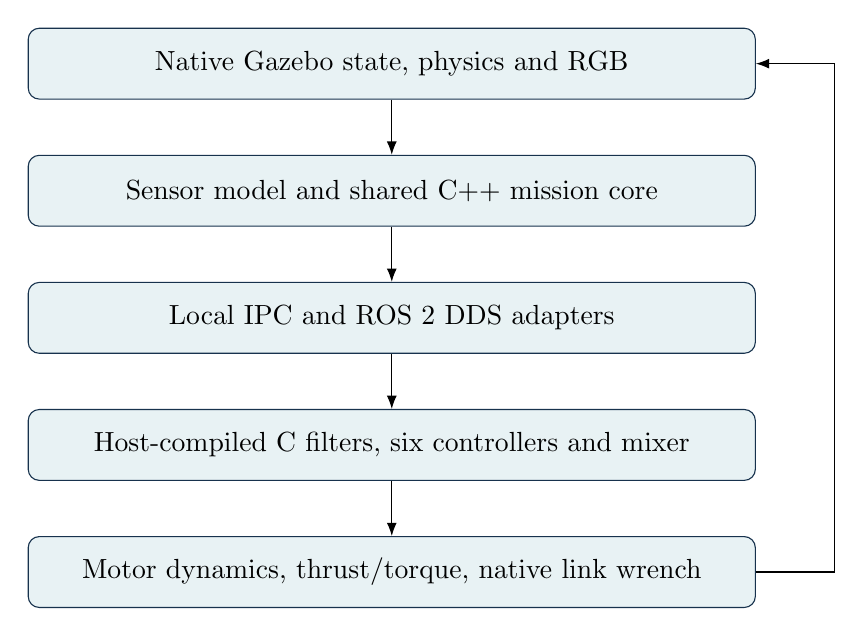
\begin{tikzpicture}[>=Latex,node distance=7mm,
box/.style={draw=ink,rounded corners,fill=soft,text width=9cm,align=center,minimum height=9mm}]
\node[box] (g){Native Gazebo state, physics and RGB};
\node[box,below=of g] (s){Sensor model and shared C++ mission core};
\node[box,below=of s] (d){Local IPC and ROS 2 DDS adapters};
\node[box,below=of d] (c){Host-compiled C filters, six controllers and mixer};
\node[box,below=of c] (m){Motor dynamics, thrust/torque, native link wrench};
\draw[->] (g)--(s);\draw[->] (s)--(d);\draw[->] (d)--(c);\draw[->] (c)--(m);
\draw[->] (m.east)--++(1,0)|-(g.east);
\end{tikzpicture}
\end{center}
The host library runs production C math, not an RP2350 emulator.
Virtual motor gating is separate from physical arming.
The recorded flight uses assumed actuator dynamics, synthetic inertial/height
observations, native camera pixels and simulated local odometry. Its downward
range is an analytical floor ray. The full standard ROS C++ graph was built and
checked separately, not silently substituted as the recorded flight path.

\section{Future physical companion}
\begin{equation*}
\text{ROS mission}\to\text{USB/UART bridge}\to\text{RP2350 parser}
\to\text{local 500 Hz control}.
\end{equation*}
Physical framing, sequence/session, CRC, freshness, status/acknowledgement,
clock handling and command authority remain work. ROS angle units are radians;
the current C interface uses degrees. Convert at one documented boundary.
A slower companion setpoint stream does not clock every inner PID iteration.

\section{Build evidence and limits}
The current simulator launcher is
\begin{quote}\ttfamily\small
powershell -ExecutionPolicy Bypass -File tools/run\_native\_garden.ps1
\end{quote}
After editing the C source, rebuild host libraries using
\texttt{tools/build\_sitl.ps1}. The separate Pico build produces ELF/UF2.
No physical board was flashed. Compilation does not prove flash durability,
sensor acquisition, telemetry delivery or actual ESC inhibition. No new flight
or implementation test suite was executed for this change.

\chapter*{References and reproducibility}
\addcontentsline{toc}{chapter}{References and reproducibility}
\begin{itemize}
\item Raspberry Pi Pico SDK flash APIs and execution safety:
\url{https://www.raspberrypi.com/documentation/pico-sdk/hardware.html}.
The installed \texttt{pico/flash.h} and linker/flash implementation were inspected.
\item NIST uncertainty evaluation:
\href{https://www.nist.gov/pml/nist-technical-note-1297}{Technical Note 1297},
\href{https://physics.nist.gov/cuu/Uncertainty/typea.html}{Type A evaluation},
\href{https://physics.nist.gov/cuu/Uncertainty/typeb.html}{Type B evaluation}.
\item ROS axes/units:
\href{https://raw.githubusercontent.com/ros-infrastructure/rep/master/rep-0103.rst}{REP 103: standard units and coordinate conventions}.
\item TDK InvenSense MPU6000/MPU6050 specification: units, noise and temperature
dependence; actual sensor configuration still needs characterization.
\item Reproducible local model calculations:
\texttt{tools/calculate\_current\_control\_design.py} and the corresponding
\texttt{artifacts/model-design/current/calculations.json}.
\item Single-file runtime source:
\texttt{flight\_controller/flight\_controller.c}.
\end{itemize}
\important{Teaching numbers and scenario coefficients are labelled assumptions.
No synthetic example is presented as measured aircraft data. Preserve raw
measurements, reference uncertainty and source/configuration with each result.}

\end{document}
